%% LyX 2.3.1 created this file.  For more info, see http://www.lyx.org/.
%% Do not edit unless you really know what you are doing.
\documentclass[english]{article}
\usepackage{fontenc}
\usepackage{inputenc}
\usepackage{graphicx}
\usepackage[top=3cm]{geometry}

\makeatletter

%%%%%%%%%%%%%%%%%%%%%%%%%%%%%% LyX specific LaTeX commands.
%% Because html converters don't know tabularnewline
\providecommand{\tabularnewline}{\\}

\@ifundefined{date}{}{\date{}}
\makeatother

\usepackage{babel}
\begin{document}
\noindent \begin{center}
\textsl{\huge{}Covered Apple Pie}{\huge\par}
\par\end{center}

\noindent \begin{center}
\textsc{Trondheim style}
\par\end{center}

\noindent \begin{center}
{\small{}Verbally transmitted from the south}{\small\par}
{\small{}\TeX ed by Lennart, translated by Stefan}{\small\par}
\par\end{center}

\begin{center}
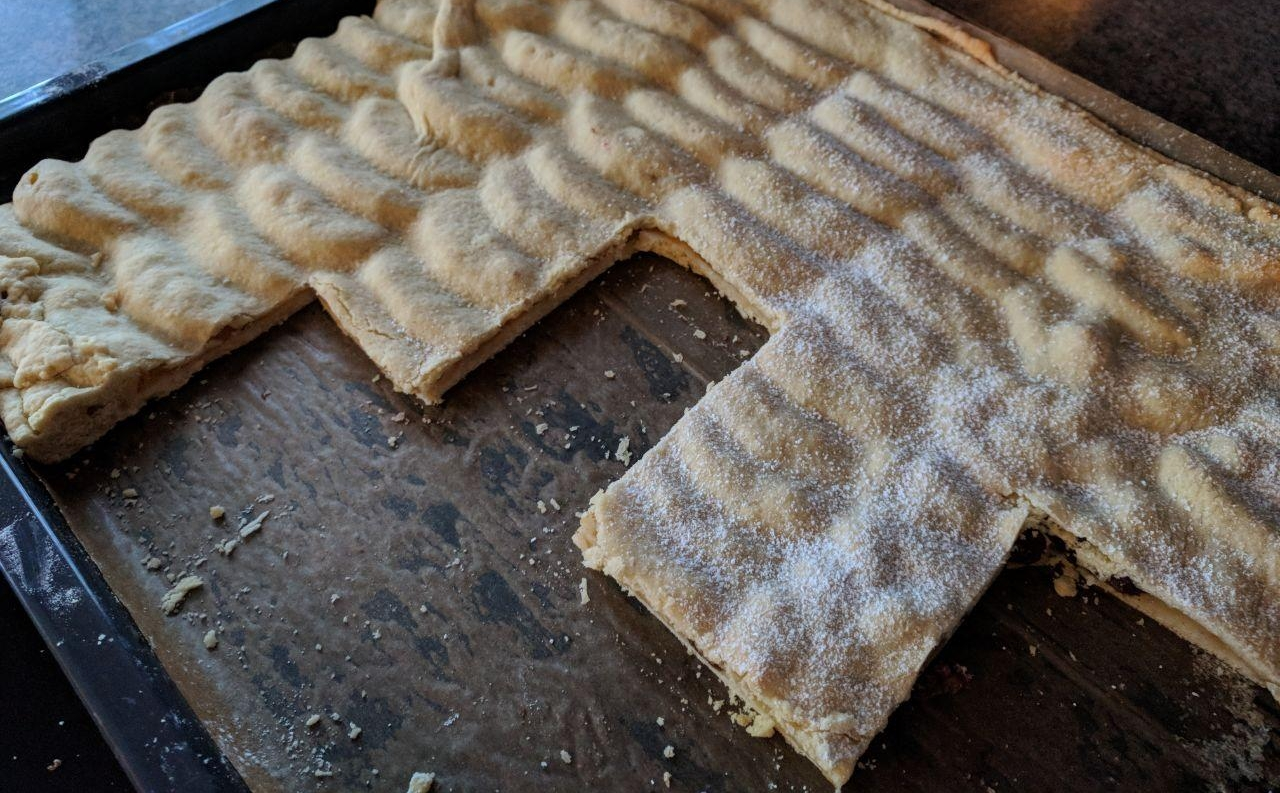
\includegraphics[width=0.6\textwidth]{cake.jpg}
\end{center}

\noindent \textbf{Ingredients }for one tray\textbf{}\\

\noindent %
\begin{tabular}{ll}
\textbf{Dough} & \tabularnewline
$375\,\mathrm{g}$ & cold butter\tabularnewline
$200\,\mathrm{g}$ & sugar\tabularnewline
$600\,\mathrm{g}$ & flour\tabularnewline
$1\,\mathrm{tea\ sp.}$ & vanilla sugar (alternatively vanilla extract or leave out)\tabularnewline
$2$ & eggs\tabularnewline
\textbf{Filling} & \tabularnewline
$10$ & small to medium apples\tabularnewline
optional & raisins\tabularnewline
optional & cinnamon\tabularnewline
\textbf{Topping} & \tabularnewline
optional & icing sugar\tabularnewline
\end{tabular}\\
\\
\textbf{}\\
\textbf{1.}\\
For the dough, mix all ingredients and knead well with hands.
Divide into two halves and chill.\\
\textbf{2.}\\
Peel 10 apples and cut them into about 12 slices per apple.\\
\textbf{3.}\\
Roll out both halves of the dough: One on the baking tray lined with baking paper,
the other one (separately) to the same size.\\
\textbf{4.}\\
Spread the apple slices on the dough on the baking tray and optionally
sprinkle them with cinnamon. Cover the cake with the other half.\\
\textbf{5.}\\
Bake at $160^{\circ}\mathrm{C}$ for about $25\,\mathrm{minutes}$
and let it cool down.\\
\textbf{6.}\\
Optionally sprinkle the finished cake with some icing sugar.
\end{document}
